A rotation matrix $^a_bR$ is an orthonormal matrix describing the rotation between two right-handed coordinate frames $\Psi_a$ and $\Psi_b$ such that any vector $^bv$ (including $\Psi_b$ coordinate axes) given in the $\Psi_b$ frame can be "rotated" into $\Psi_a$ coordinates by the operation
\begin{equation}
^av =\, ^a_bR \,\,^bv
\end{equation}
Note that the matrix $^a_bR$ can also be seen as the rotation required of the frame $\Psi_a$ for it to coincide with $\Psi_b$.
Rotation of the frame $\Psi_a$ with an angle $\theta$ counterclockwise about a single axis (equal to clockwise "rotation" of the any vector in $\Psi_b$) correspond to the rotation matrices
\begin{equation}
^a_bR_x = 
\begin{bmatrix}
1 & 0 & 0\\
0 & \cos\theta & -\sin\theta\\
0 & \sin\theta & \cos\theta
\end{bmatrix} 
\qquad
^a_bR_y = 
\begin{bmatrix}
\cos\theta & 0 & \sin\theta \\
0 & 1 & 0\\
-\sin\theta & 0 & \cos\theta
\end{bmatrix}
\qquad
^a_bR_z = 
\begin{bmatrix}
\cos\theta & -\sin\theta & 0\\
\sin\theta & \cos\theta & 0\\
0 & 0 & 1
\end{bmatrix}
\end{equation}

The translation of the origin from the coordinate system $\Psi_a$ to $\Psi_b$ can be described by the position vector $^a_bp$, which is a vector given in the $\Psi_a$ coordinate frame.
The relative configuration of two coordinate frames is their relative position and orientation, which can be expressed expressed by a homogeneous matrix
\begin{equation}
^a_bH = 
\begin{bmatrix}
^a_bR & ^a_bp\\
0 & 1
\end{bmatrix}
\end{equation}


The position of the end-effector (the tip of the instrument) given in an inertial frame, can be described as a sequence of joint rotations of the robot and and instrument, and translation from the inertial origin via the fixed-length links and the slide of the instrument.

A coordinate frame is defined for each degree of freedom, with origin in the center of rotation. 








The clockwise rotation of the frame $\Psi_a$ to coincide with the frame $\Psi_b$ corresponds to the counterclockwise rotation of the vector $^bv$ which will transform it to $\Psi_a$ coordinates. The inverse of a rotation matrix (rotation in the opposite direction) is its transpose.


\section{Robot Hand Kinematics}
Illustration of robotic arm and definition of coordinate frames of outer part of the arm incl hand/wrist/gripper. Can we define kinematic and dynamic equations?

\begin{figure}[htbp]
	\hspace{-15mm}
	\subbottom[Coordinate frames for the joints on the robot "hand".]{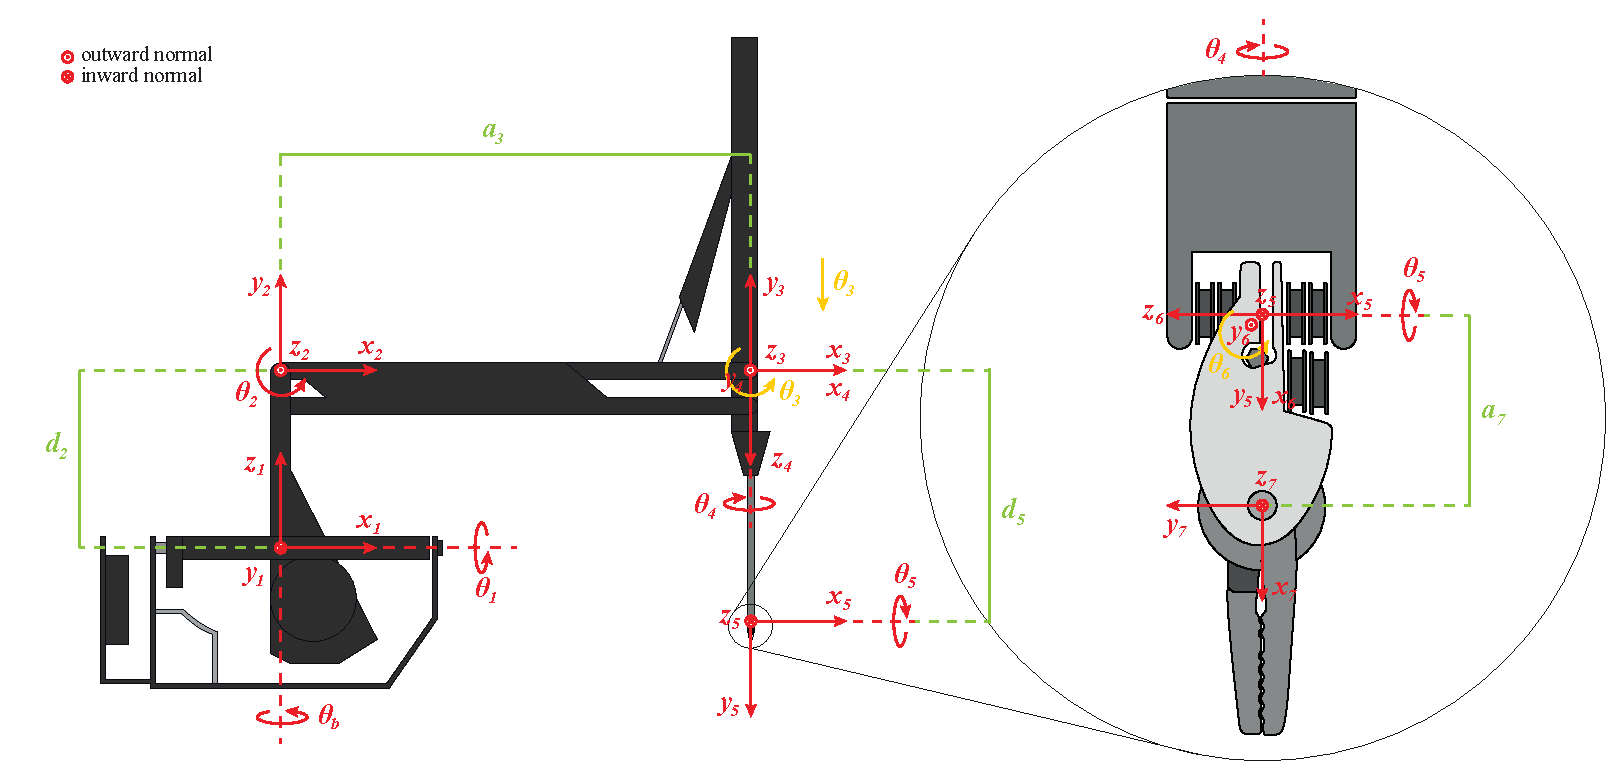
\includegraphics[width=1.2\textwidth]{robot_coordinate_systems.pdf}\label{fig:robot_coordinate_systems}}%
	\vspace{1mm}
	\subbottom[The\,\,da\,\,Vinci\,\,inertial\,\,frame.]{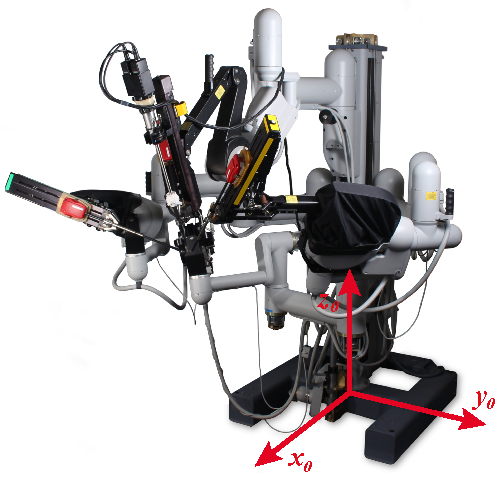
\includegraphics[height=5.1cm]{robot_base_frame1.pdf}\label{fig:robot_base_frame}}%
	\hspace{10mm}
	\subbottom[Robot arm (grey) with inertial and robot hand base frame.]{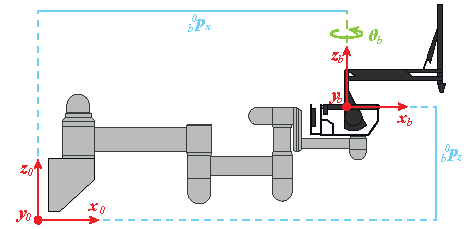
\includegraphics[height=4.7cm]{robot_arm_with_frames.pdf}\label{fig:robot_arm_with_frames}}%
	\caption{.}
	\label{fig:robot_frames}
\end{figure}

The inertial reference frame $\Psi_0$ is fixed with its origin at the robot base, as seen in \autoref{fig:robot_base_frame}. Assuming all arm joints (grey part of \autoref{fig:robot_arm_with_frames}) have zero angle, the configuration of the robot base frame (the joint of attachment between robot arm and robot hand) given in the inertial coordinates, is a pure translation along the inertial $x$- and $z$-axes:
\begin{equation}
^0_b T = \begin{bmatrix}
1 & 0 & 0 & ^0_bp_x\\
0 & 1 & 0 & 0\\
0 & 0 & 1 & ^0_bp_z\\
0 & 0 & 0 & 1
\end{bmatrix}
\end{equation}

The configuration of the first link frame $\Psi_1$ given in the base frame coordinates is identity, and the joint can be rotated some $\theta_1$ about the frame $z$-axis (see \autoref{fig:robot_coordinate_systems} and \ref{fig:robot_arm_with_frames}), giving the configuration matrix:
\begin{equation}
^b_1 T(\theta_1) = 
\begin{bmatrix}
\cos\theta_1 & -\sin\theta_1 & 0 & 0\\
\sin\theta_1 & \cos\theta_1 & 0 & 0\\
0 & 0 & 1 & 0\\
0& 0& 0& 1
\end{bmatrix}
\end{equation}

To get to the second link frame $\Psi_2$, the first frame is rotated 90$^\circ$ about its $x$-axis, and the joint can be rotated some $\theta_2$ about its $x$-axis. Finally the origin of the second link frame is displaced with a distance $d_2$ from the first link frame along its $z$-axis:
\begin{equation}
^1_2 T(\theta_2) = 
\begin{bmatrix}
1 & 0 & 0 & 0\\
0 & 0 & -1 & 0\\
0 & 1 & 0 & 0\\
0 & 0 &  0 & 1
\end{bmatrix} 
\begin{bmatrix}
1 & 0 & 0 & 0\\
0 & \cos\theta & -\sin\theta & 0\\
0 & \sin\theta & \cos\theta & 0\\
 0 & 0 & 0 & 1
\end{bmatrix}  
=
\begin{bmatrix}
1 & 0 & 0 & 0\\
0 & -\sin\theta_2 & -\cos\theta_2 & 0\\
0 & \cos\theta_2 & -\sin\theta_2 & 0\\
0 & 0 &  0 & 1
\end{bmatrix}
\neq
\begin{bmatrix}
\cos\theta_1 & -\sin\theta_1 & 0 & 0\\
\sin\theta_1 & \cos\theta_1 & 0 & 0\\
0 & 0 & 1 & 0\\
0& 0& 0& 1
\end{bmatrix}
\end{equation}

\section{Beating Heart Dynamic Model}
Illustration of heart model and description of kinematics and dynamics.
Quasi-periodic rigid 3D motion, combination of two periodic motions \cite{bib:heart_berkeley}. Frequencies assumed known from ECG and mechanical ventilator.

"The estimated components are then combined to predict future motion of the heart surface. This information, in turn, is used in the design of an explicit controller that stabilizes the relative motion of a surgical tool to a desired distance and orientation with respect to the heart surface."

"We then present a control law that uses the predicted motion to asymptotically stabilize the motion of the surgical tool to a desired distance and orientation with respect to the heart surface."

"To simplify the analysis and allow real-time prediction, we do not take the cause of the motion into consideration, and only consider the kinematics of a local area of interest on the heart surface."

"Fortunately, in this application, we have a reasonably good estimate of the phase1 and frequency of the two motion components: the respiratory phase and frequency can be obtained from the mechanical ventilator, and the cardiac phase and frequency are detected by an ECG monitor."

"choosing a convenient initial position and orientation for $\Psi_d$, e.g. such that $p^d_h(0)=0$ and $R^0_d(0) = I$

Relative configuration between heart and robot tool $H^h_r$ (with $R^h_r =[r_x, r_y, r_z]$) and error function $J(H^h_r)$
\begin{equation}
J(H^h_r) = \underbrace{\tfrac{1}{2}k_p (p^h_r-\Delta r_z)^T(p^h_r-\Delta r_z)}_\text{translational error} + \underbrace{k_x (1-e_x^T r_x) + k_y (1-e_y^T r_y) + k_z (1-e_z^T r_z)}_\text{rotational error}
\end{equation}
\begin{tabular}{rl}
	where &\\
	$\Delta$ & is the desired relative distance between the tool and the heart\\
	$E=[e_x,e_y,e_z]$ & is a rotation matrix describing the desired orientation of the tool frame\\
	$k_p,k_x,k_y,k_z$ & are constant positive parameters\\
\end{tabular}\\

Then $J$ is equal to zero (has its minimum) only when $p^h_r=\Delta r_z$ (the origin of $\Psi_r$ given in h coordinates is $\Delta$ away from the origin of $Psi_h$ along the surface normal) and $R^h_r=E$ (frame h and r axes are aligned).
\begin{align}
\dot{J} &= 
\begin{bmatrix}
k_x \hat{e}_x r_x + k_y \hat{e}_y r_y + k_z \hat{e}_z r_z\\
k_p(p^h_r - \Delta r_z)
\end{bmatrix}^T
\begin{bmatrix}
\omega^{h,h}_r \\
r^{h,h}_r
\end{bmatrix}
= (dJ)^T T^{h,h}_r\\
\dot{H}^h_r &= 
\begin{bmatrix}
\hat{\omega}^{h,h}_r r_x & \hat{\omega}^{h,h}_r r_y & \hat{\omega}^{h,h}_r r_z & \hat{\omega}^{h,h}_r p^h_r + v^{h,h}_r\\
0 & 0 & 0 & 0
\end{bmatrix}\\
(\dot{dJ}) &=
\begin{bmatrix}
-k_x \hat{e}_x \hat{r}_x  - k_y \hat{e}_y \hat{r}_y - k_z \hat{e}_z \hat{r}_z & 0\\
-k_p(\hat{p}^h_r - \Delta \hat{r}_z) & k_p I
\end{bmatrix}
T^{h,h}_r
\end{align}

"We do not consider specific robot dynamics at this point and only specify the desired inertial acceleration $\dot{T}^{0,0}_r$ of the robot end effector frame $\Psi_r$. Proposed desired acceleration"
\begin{equation}
\left(\dot{T}^{0,0}_r\right)_\text{des} = \dot{T}^{0,0}_h - \text{Ad}_{H^0_h} K_1 (\dot{dJ}) + \text{ad}_{T^{0,0}_h} T^{0,h}_r - \text{Ad}_{H^0_h} K_2 (T^{h,h}_r + K_1 dJ)
\end{equation}
\begin{tabular}{rl}
	where & \\
	$K1, K_2$ & are symmetric and positive definite matrices\\
	$H^0_h$ & is the estimated configuration of the frame $\Psi_h$ at the area of interest on the heart surface\\
	$T^{0,0}_h$ & is the estimated velocity of the frame $\Psi_h$ at the area of interest on the heart surface\\
	$\dot{T}^{0,0}_h$ & is the estimated acceleration of the frame $\Psi_h$ at the area of interest on the heart surface\\
\end{tabular}\\

This controller drives $T^{h,h}_r$ to $-K_1dJ$ by the gain $K_2$, along the steepest descend of $J$. Asymptotic stability at $J=0$, with Lyapunov function
\begin{equation}
V=\kappa_1 J + \tfrac{1}{2} (T^{h,h}_r + K_1dJ)^T K_2^{-1}(T^{h,h}_r + K_1dJ)
\end{equation}
\begin{tabular}{rl}
	where & \\
	$\kappa_1$ & is a positive constant strictly less than 4 times the smallest singular value of $K_1$, $0<\kappa_1 <4\sigma_\text{min}(K_1)$
\end{tabular}

Assuming the robot achieves perfect tracking of $\left(\dot{T}^{0,0}_r\right)_\text{des}$, the time derivative of $V$ along the system trajectories is
\begin{equation}
\dot{V} = -\left(T^{h,h}_r + (K_1 - \tfrac{\kappa_1}{2}I)dJ\right)^T \left(T^{h,h}_r + (K_1 - \tfrac{\kappa_1}{2}I)dJ\right) - \kappa_1(dJ ^T(K_1 - \tfrac{\kappa_1}{4}I)dJ
\end{equation}
\begin{tabular}{rl}
	where & \\
	$I$ & is the identity matrix\\
	$K_1 - \tfrac{\kappa_1}{4}$ & is strictly positive because of the choice of $\kappa_1$\\
\end{tabular}